% Options for packages loaded elsewhere
\PassOptionsToPackage{unicode}{hyperref}
\PassOptionsToPackage{hyphens}{url}
\PassOptionsToPackage{dvipsnames,svgnames,x11names}{xcolor}
%
\documentclass[
]{hdsr}

\usepackage{amsmath,amssymb}
\usepackage{iftex}
\ifPDFTeX
  \usepackage[T1]{fontenc}
  \usepackage[utf8]{inputenc}
  \usepackage{textcomp} % provide euro and other symbols
\else % if luatex or xetex
  \usepackage{unicode-math}
  \defaultfontfeatures{Scale=MatchLowercase}
  \defaultfontfeatures[\rmfamily]{Ligatures=TeX,Scale=1}
\fi
\usepackage{lmodern}
\ifPDFTeX\else  
    % xetex/luatex font selection
\fi
% Use upquote if available, for straight quotes in verbatim environments
\IfFileExists{upquote.sty}{\usepackage{upquote}}{}
\IfFileExists{microtype.sty}{% use microtype if available
  \usepackage[]{microtype}
  \UseMicrotypeSet[protrusion]{basicmath} % disable protrusion for tt fonts
}{}
\makeatletter
\@ifundefined{KOMAClassName}{% if non-KOMA class
  \IfFileExists{parskip.sty}{%
    \usepackage{parskip}
  }{% else
    \setlength{\parindent}{0pt}
    \setlength{\parskip}{6pt plus 2pt minus 1pt}}
}{% if KOMA class
  \KOMAoptions{parskip=half}}
\makeatother
\usepackage{xcolor}
\setlength{\emergencystretch}{3em} % prevent overfull lines
\setcounter{secnumdepth}{-\maxdimen} % remove section numbering
% Make \paragraph and \subparagraph free-standing
\ifx\paragraph\undefined\else
  \let\oldparagraph\paragraph
  \renewcommand{\paragraph}[1]{\oldparagraph{#1}\mbox{}}
\fi
\ifx\subparagraph\undefined\else
  \let\oldsubparagraph\subparagraph
  \renewcommand{\subparagraph}[1]{\oldsubparagraph{#1}\mbox{}}
\fi


\providecommand{\tightlist}{%
  \setlength{\itemsep}{0pt}\setlength{\parskip}{0pt}}\usepackage{longtable,booktabs,array}
\usepackage{calc} % for calculating minipage widths
% Correct order of tables after \paragraph or \subparagraph
\usepackage{etoolbox}
\makeatletter
\patchcmd\longtable{\par}{\if@noskipsec\mbox{}\fi\par}{}{}
\makeatother
% Allow footnotes in longtable head/foot
\IfFileExists{footnotehyper.sty}{\usepackage{footnotehyper}}{\usepackage{footnote}}
\makesavenoteenv{longtable}
\usepackage{graphicx}
\makeatletter
\def\maxwidth{\ifdim\Gin@nat@width>\linewidth\linewidth\else\Gin@nat@width\fi}
\def\maxheight{\ifdim\Gin@nat@height>\textheight\textheight\else\Gin@nat@height\fi}
\makeatother
% Scale images if necessary, so that they will not overflow the page
% margins by default, and it is still possible to overwrite the defaults
% using explicit options in \includegraphics[width, height, ...]{}
\setkeys{Gin}{width=\maxwidth,height=\maxheight,keepaspectratio}
% Set default figure placement to htbp
\makeatletter
\def\fps@figure{htbp}
\makeatother
\newlength{\cslhangindent}
\setlength{\cslhangindent}{1.5em}
\newlength{\csllabelwidth}
\setlength{\csllabelwidth}{3em}
\newlength{\cslentryspacingunit} % times entry-spacing
\setlength{\cslentryspacingunit}{\parskip}
\newenvironment{CSLReferences}[2] % #1 hanging-ident, #2 entry spacing
 {% don't indent paragraphs
  \setlength{\parindent}{0pt}
  % turn on hanging indent if param 1 is 1
  \ifodd #1
  \let\oldpar\par
  \def\par{\hangindent=\cslhangindent\oldpar}
  \fi
  % set entry spacing
  \setlength{\parskip}{#2\cslentryspacingunit}
 }%
 {}
\usepackage{calc}
\newcommand{\CSLBlock}[1]{#1\hfill\break}
\newcommand{\CSLLeftMargin}[1]{\parbox[t]{\csllabelwidth}{#1}}
\newcommand{\CSLRightInline}[1]{\parbox[t]{\linewidth - \csllabelwidth}{#1}\break}
\newcommand{\CSLIndent}[1]{\hspace{\cslhangindent}#1}

%Graphics should all go in the figs/ directory
\graphicspath{{figs/}}
\makeatletter
\makeatother
\makeatletter
\makeatother
\makeatletter
\@ifpackageloaded{caption}{}{\usepackage{caption}}
\AtBeginDocument{%
\ifdefined\contentsname
  \renewcommand*\contentsname{Table of contents}
\else
  \newcommand\contentsname{Table of contents}
\fi
\ifdefined\listfigurename
  \renewcommand*\listfigurename{List of Figures}
\else
  \newcommand\listfigurename{List of Figures}
\fi
\ifdefined\listtablename
  \renewcommand*\listtablename{List of Tables}
\else
  \newcommand\listtablename{List of Tables}
\fi
\ifdefined\figurename
  \renewcommand*\figurename{Figure}
\else
  \newcommand\figurename{Figure}
\fi
\ifdefined\tablename
  \renewcommand*\tablename{Table}
\else
  \newcommand\tablename{Table}
\fi
}
\@ifpackageloaded{float}{}{\usepackage{float}}
\floatstyle{ruled}
\@ifundefined{c@chapter}{\newfloat{codelisting}{h}{lop}}{\newfloat{codelisting}{h}{lop}[chapter]}
\floatname{codelisting}{Listing}
\newcommand*\listoflistings{\listof{codelisting}{List of Listings}}
\makeatother
\makeatletter
\@ifpackageloaded{caption}{}{\usepackage{caption}}
\@ifpackageloaded{subcaption}{}{\usepackage{subcaption}}
\makeatother
\makeatletter
\makeatother
\ifLuaTeX
  \usepackage{selnolig}  % disable illegal ligatures
\fi
\IfFileExists{bookmark.sty}{\usepackage{bookmark}}{\usepackage{hyperref}}
\IfFileExists{xurl.sty}{\usepackage{xurl}}{} % add URL line breaks if available
\urlstyle{same} % disable monospaced font for URLs
\hypersetup{
  pdftitle={A Very Enticing Title},
  pdfauthor={First Author; Second Author; Second Author; Third Author},
  pdfkeywords={up, to, six, keywords},
  colorlinks=true,
  linkcolor={blue},
  filecolor={Maroon},
  citecolor={Blue},
  urlcolor={Blue},
  pdfcreator={LaTeX via pandoc}}

\title{A Very Enticing Title}
\author{First Author \and Second Author \and Second Author \and Third
Author}
\date{}

\begin{document}
\maketitle
\begin{abstract}
The abstract should be no more than 250 words.
\end{abstract}
\hypertarget{media-summary}{%
\subsection*{Media Summary}\label{media-summary}}
\addcontentsline{toc}{subsection}{Media Summary}

The Media Summary should be written in plain language to highlight the
key messages of the article, in ways that can be understood by the
general public and cited by the media directly and accurately. It
therefore should avoid technical terms or language designed for academic
communications. It should not exceed 400 words, and more succinct, the
better.

\hypertarget{sec-sec1}{%
\subsection{An Informative Section Title}\label{sec-sec1}}

Because we use section titles in a pull-down menu for the online version
as signposts, please use as specific and informative titles as possible.
Avoid generic section titles such as
\texttt{methods,\textquotesingle{}\textquotesingle{}}data,'\,' and
\texttt{results\textquotesingle{}\textquotesingle{}.\ Such\ titles\ are\ common\ in\ certain\ technical\ journals,\ but\ they\ do\ not\ work\ well\ for\ HDSR,\ which\ aims\ to\ publish}everything
data science and data science for everyone''. Try to use titles that
will make readers (and you!) think that
\texttt{Hmmm,\ that\ sounds\ interesting\textquotesingle{}\textquotesingle{}\ or}Hmmm,
that's unexpected and I better to take a look.'\,' The same goes with
the article title, and indeed the entire article. Considering you are
not writing a technical article, but rather telling a data science story
with layered plots, an enticing flow, and a memorable punch line. That
is, an article you want to read, and will walk away feeling ``Wow, that
was inspiring -- I never thought about that!'\,'

\[
    i\hbar \frac{\partial \Psi}{\partial t} = -\frac{\hbar^2}{2m}\frac{\partial^2 \Psi}{\partial x^2} + V \Psi
\]

\hypertarget{subsection}{%
\subsubsection{Subsection}\label{subsection}}

Building upon previous work by Murray (2020), dolor sit amet,
consectetur adipiscing elit. Pellentesque id massa vulputate, tristique
mi id, imperdiet mi.

\hypertarget{section-title}{%
\subsection{Section title}\label{section-title}}

Lorem ipsum dolor sit amet, consectetur adipiscing elit. Pellentesque id
massa vulputate, tristique mi id, imperdiet mi. Mauris id ante ac lacus
mollis sagittis. Sed imperdiet nibh id eros malesuada, at fermentum urna
mollis. Sed id elit eu arcu varius tempor tincidunt in orci. Nullam
accumsan diam vitae nibh fermentum, nec facilisis leo pulvinar. Ut
condimentum nisl in orci euismod mattis. Fusce at mauris augue.

\hypertarget{section-title-1}{%
\subsection{Section title}\label{section-title-1}}

Lorem ipsum dolor sit amet, consectetur adipiscing elit. Pellentesque id
massa vulputate, tristique mi id, imperdiet mi. Mauris id ante ac lacus
mollis sagittis. Sed imperdiet nibh id eros malesuada, at fermentum urna
mollis.

\[
-\frac{\hbar^2}{2m} \frac{d^2 \psi}{dx^2} + V\psi = E\psi\\
\]

Sed id elit eu arcu varius tempor tincidunt in orci. Nullam accumsan
diam vitae nibh fermentum, nec facilisis leo pulvinar. Ut condimentum
nisl in orci euismod mattis. Fusce at mauris augue.

\begin{figure}

{\centering 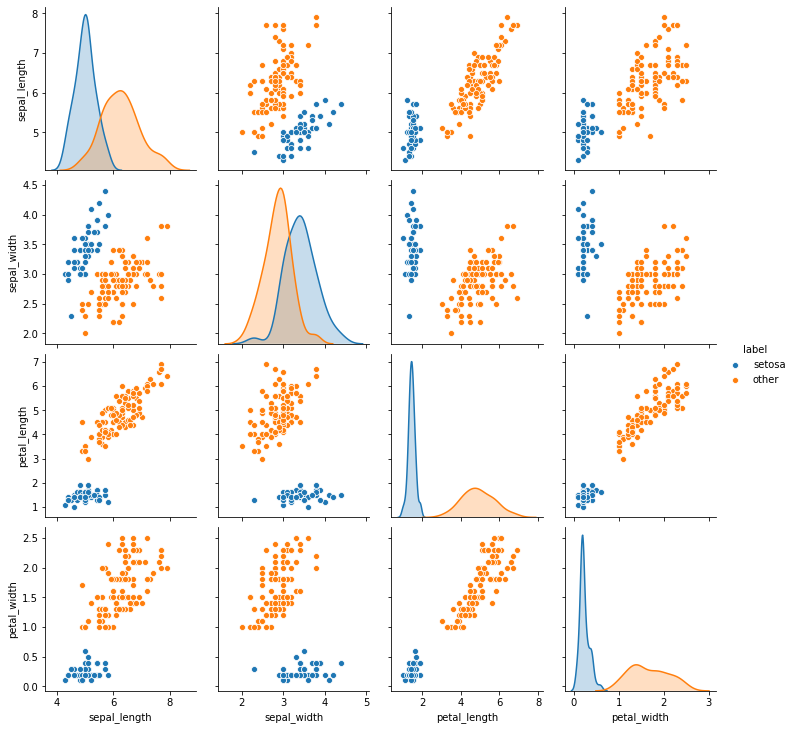
\includegraphics{figs/iris_pairs.png}

}

\caption{\label{fig-my-label}This is an example figure.}

\end{figure}

\hypertarget{disclosure-statement}{%
\subsubsection*{Disclosure Statement}\label{disclosure-statement}}
\addcontentsline{toc}{subsubsection}{Disclosure Statement}

The authors have no conflicts of interest to declare.

\hypertarget{acknowledgments}{%
\subsubsection*{Acknowledgments}\label{acknowledgments}}
\addcontentsline{toc}{subsubsection}{Acknowledgments}

Lorem ipsum dolor sit amet, consectetur adipiscing elit. Pellentesque id
massa vulputate, tristique mi id, imperdiet mi. Mauris id ante ac lacus
mollis sagittis. Sed imperdiet nibh id eros malesuada, at fermentum urna
mollis. Sed id elit eu arcu varius tempor tincidunt in orci. Nullam
accumsan diam vitae nibh fermentum, nec facilisis leo pulvinar. Ut
condimentum nisl in orci euismod mattis. Fusce at mauris augue.

\hypertarget{contributions}{%
\subsubsection*{Contributions}\label{contributions}}
\addcontentsline{toc}{subsubsection}{Contributions}

Lorem ipsum dolor sit amet, consectetur adipiscing elit. Pellentesque id
massa vulputate, tristique mi id, imperdiet mi. Mauris id ante ac lacus
mollis sagittis. Sed imperdiet nibh id eros malesuada, at fermentum urna
mollis. Sed id elit eu arcu varius tempor tincidunt in orci. Nullam
accumsan diam vitae nibh fermentum, nec facilisis leo pulvinar. Ut
condimentum nisl in orci euismod mattis. Fusce at mauris augue.

\hypertarget{sec-appendix-customize-this-label}{%
\subsection{Title}\label{sec-appendix-customize-this-label}}

Lorem ipsum dolor sit amet, consectetur adipiscing elit. Pellentesque id
massa vulputate, tristique mi id, imperdiet mi. Mauris id ante ac lacus
mollis sagittis. Sed imperdiet nibh id eros malesuada, at fermentum urna
mollis. Sed id elit eu arcu varius tempor tincidunt in orci.

\[
e^{i\theta} = \cos \theta + i\sin \theta
\]

Nullam accumsan diam vitae nibh fermentum, nec facilisis leo pulvinar.
Ut condimentum nisl in orci euismod mattis. Fusce at mauris augue.

\hypertarget{bibliography}{%
\section*{References}\label{bibliography}}
\addcontentsline{toc}{section}{References}

\hypertarget{refs}{}
\begin{CSLReferences}{1}{0}
\leavevmode\vadjust pre{\hypertarget{ref-2020.03.27.20043752}{}}%
Murray, Christopher JL. 2020. {``Forecasting {COVID-19} Impact on
Hospital Bed-Days, {ICU}-Days, Ventilator-Days and Deaths by {US} State
in the Next 4 Months.''} \emph{medRxiv}.
\url{https://doi.org/10.1101/2020.03.27.20043752}.

\end{CSLReferences}



\end{document}
